
In this section we want to show and evaluate our results.

\subsection{\co emissions per sector}

\subsubsection{Power industry results}
Depending on the country we are studying, the obtained correlation is very different. 

In Figure \ref{fig:indicators_EEUU_China} we have two cases with only two indicators: United States and China. In the first one we got a correlation larger than 0.8, while in China it does not reach 0.1.
\begin{figure}[h!]
	\centering
	\subfloat[United States]{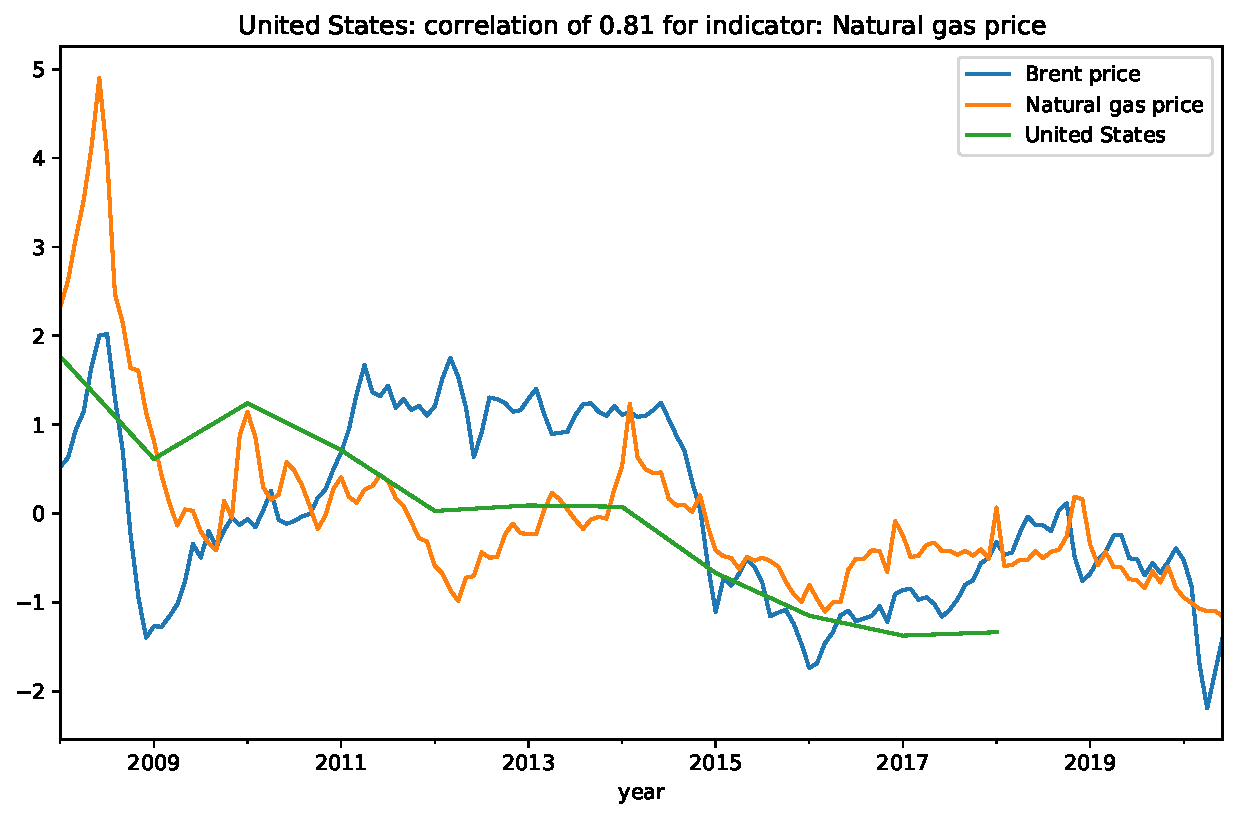
\includegraphics[width=0.5\linewidth]{../power_industry/United States_indicators}}
	\subfloat[China]{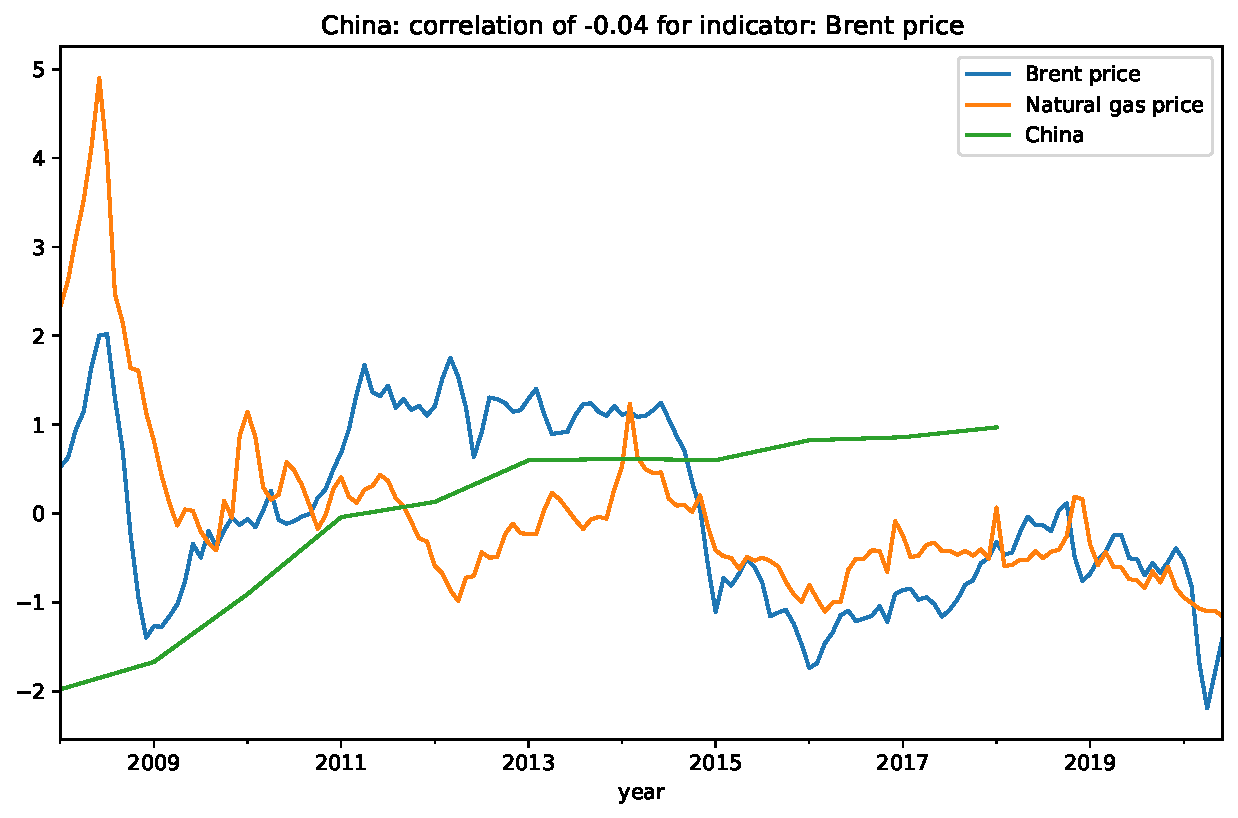
\includegraphics[width=0.5\linewidth]{../power_industry/China_indicators}}
	\caption{Indicators and annual emissions for non European countries.}
	\label{fig:indicators_EEUU_China}
\end{figure}

The same behavior appears in European countries where we have 4 indicators as it is shown in the Figure \ref{fig:indicators_Denmark_Portugal}
\begin{figure}[h!]
	\centering
	\subfloat[Denmark]{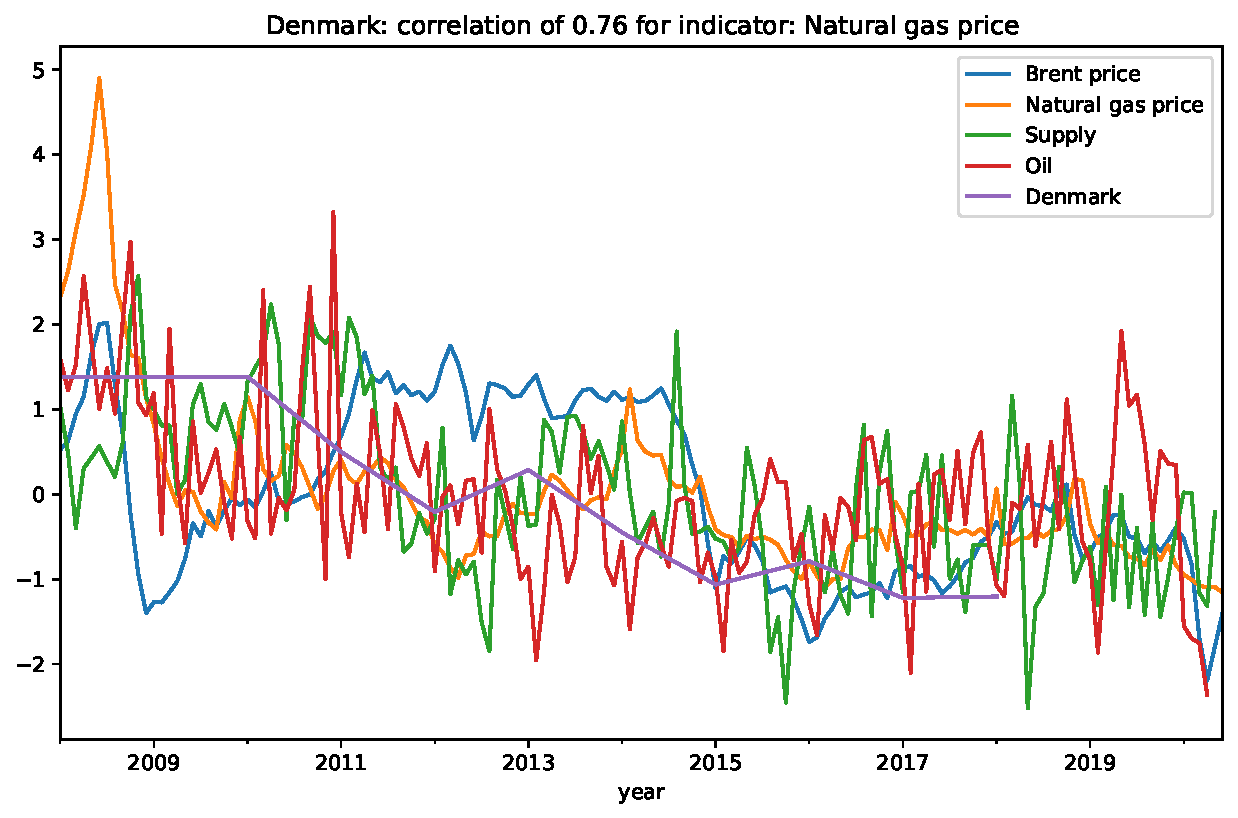
\includegraphics[width=0.5\linewidth]{../power_industry/Denmark_indicators}}
	\subfloat[Portugal]{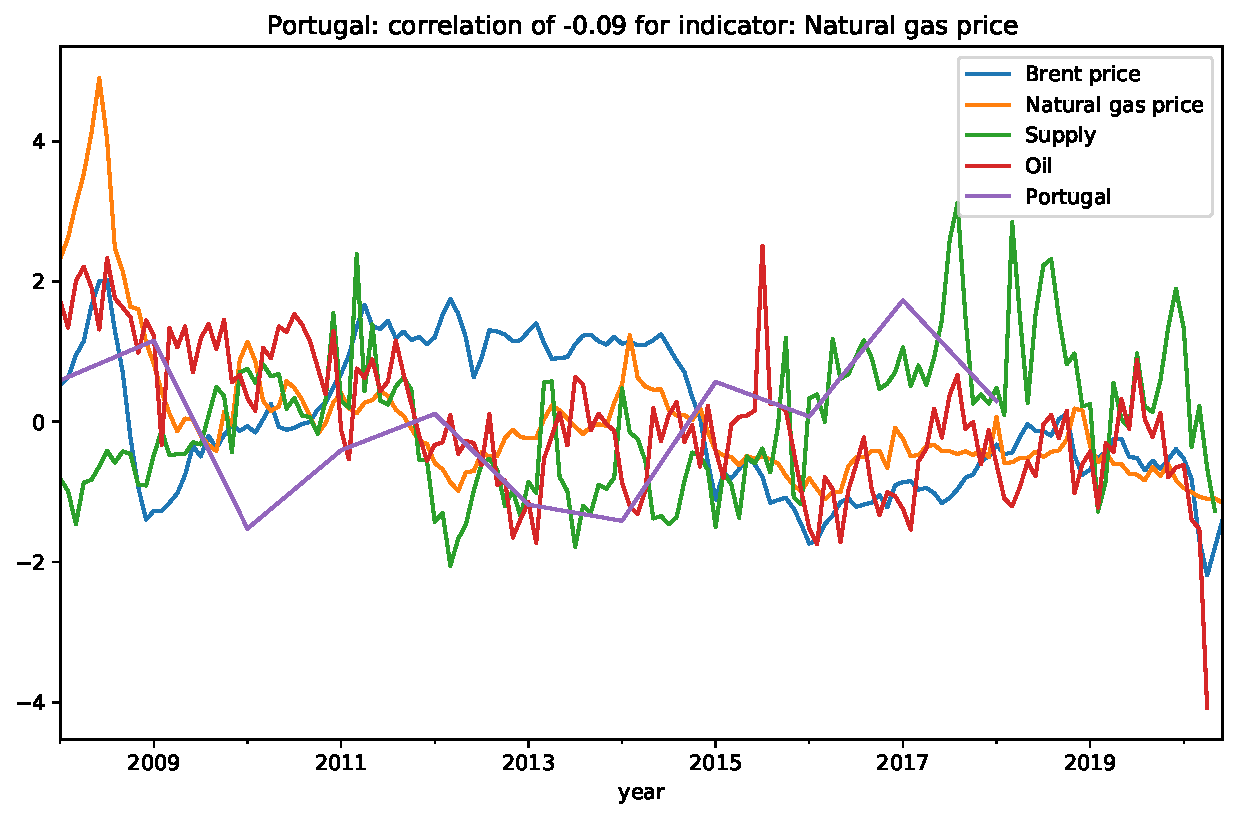
\includegraphics[width=0.5\linewidth]{../power_industry/Portugal_indicators}}
	\caption{Indicators and annual emissions for European countries.}
	\label{fig:indicators_Denmark_Portugal}
\end{figure}

In Table \ref{table:correlation} we can observe the selected indicators and the respective correlation with the emissions for the 8 biggest contributors in emissions.
\begin{table}[h!]
	\centering
	\begin{tabular}{ccc}
		\hline
		Country & Correlation Indicator \& Emissions & Selected Indicator \\
		\hline
		\hline 
		EU & 0.740 & Brent Price \\
		United States & 0.813 & Natural Gas Price \\
		India & -0.272 & Brent Price \\
		China & -0.038 &  Brent Price \\
		Japan &  0.428 & Brent Price \\
		Russia & 0.792 & Brent Price \\
		Canada & 0.785 & Natural Gas Price \\
		Brazil & 0.021 & Brent Price\\
		\hline 
		&& \\
	\end{tabular}
	\caption{Resulting correlations for the biggest contributors}
	\label{table:correlation}  
\end{table}

Once the indicator is selected, SARIMA model is applied per country, allowing us to check if there is a relative change in this indicator and simultaneously to $ CO_2 $ emissions. The results are plotted in Figure \ref{fig:sarima}. 
\begin{figure}[h!]
	\centering
	\subfloat[European Union]{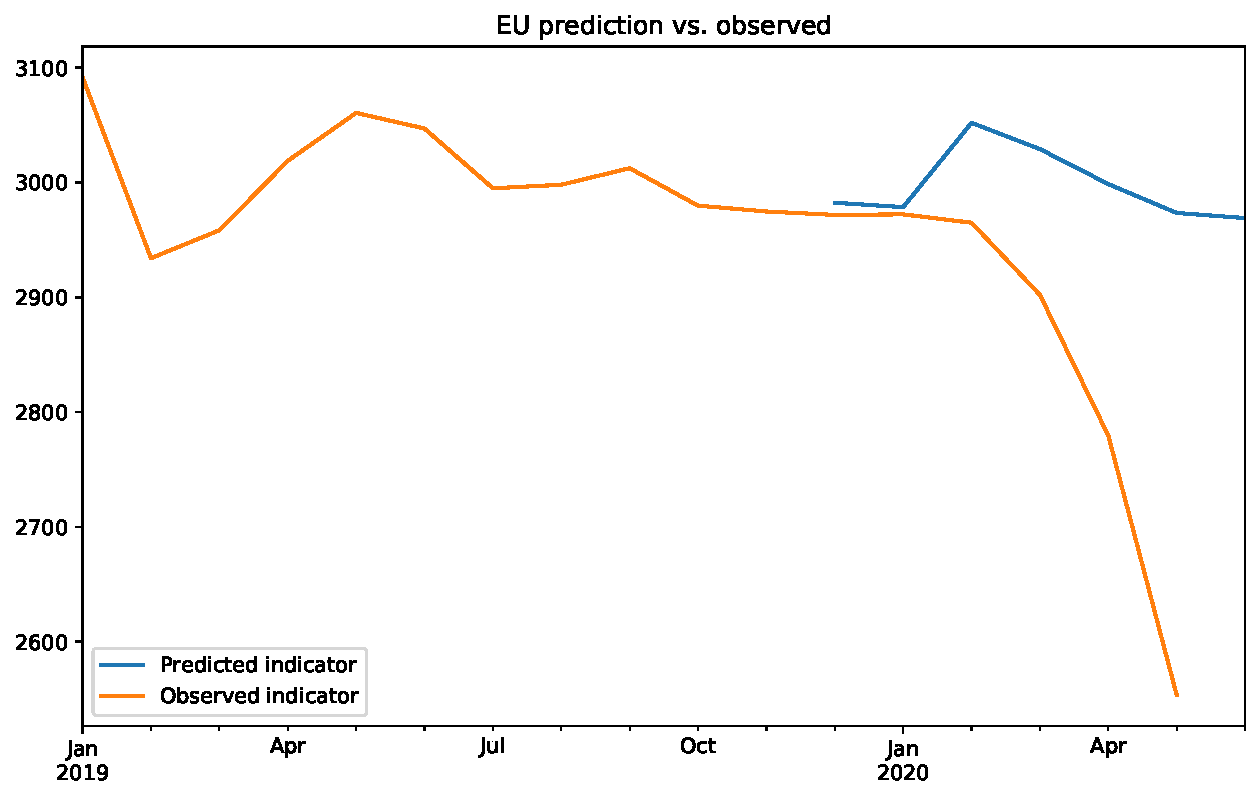
\includegraphics[width=0.4\linewidth]{../power_industry/EU_prediction}}
	\subfloat[United States]{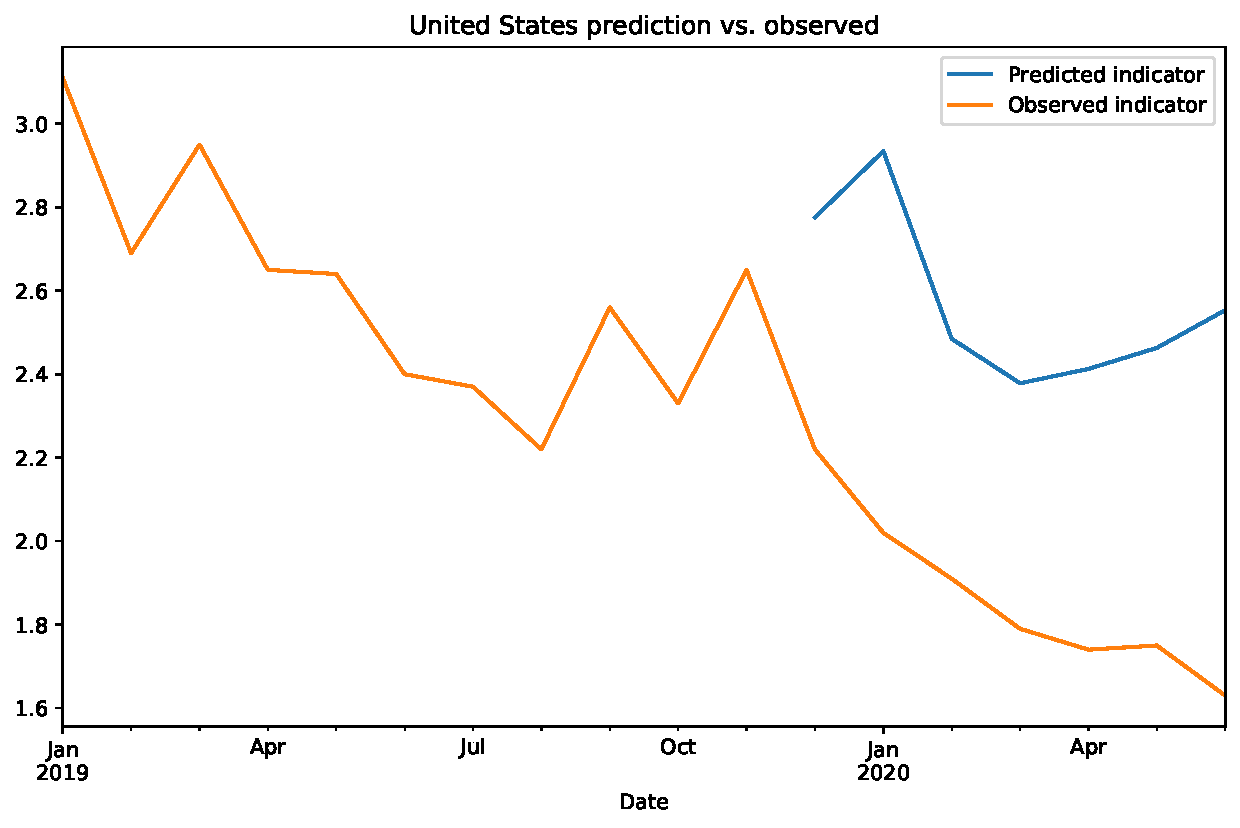
\includegraphics[width=0.4\linewidth]{../power_industry/United States_prediction}} \\
	\subfloat[India]{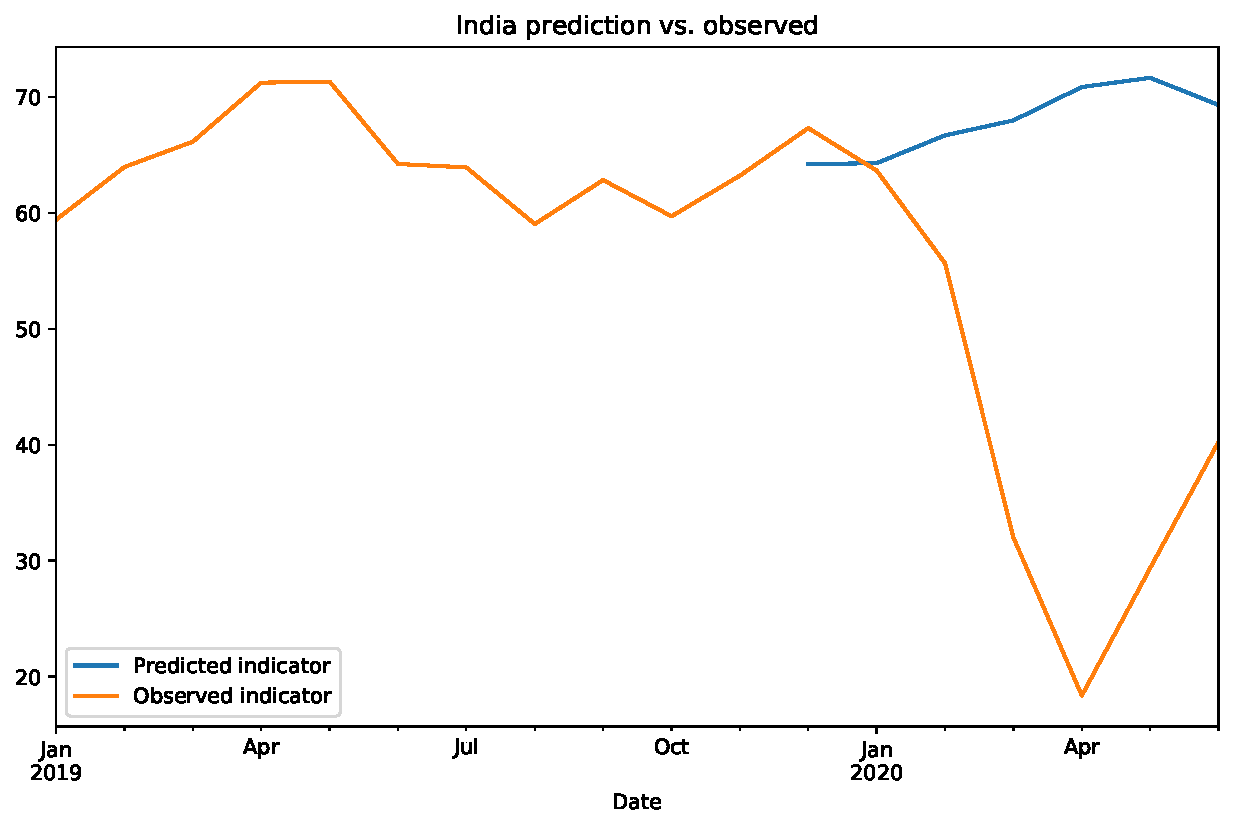
\includegraphics[width=0.4\linewidth]{../power_industry/India_prediction}}
	\subfloat[China]{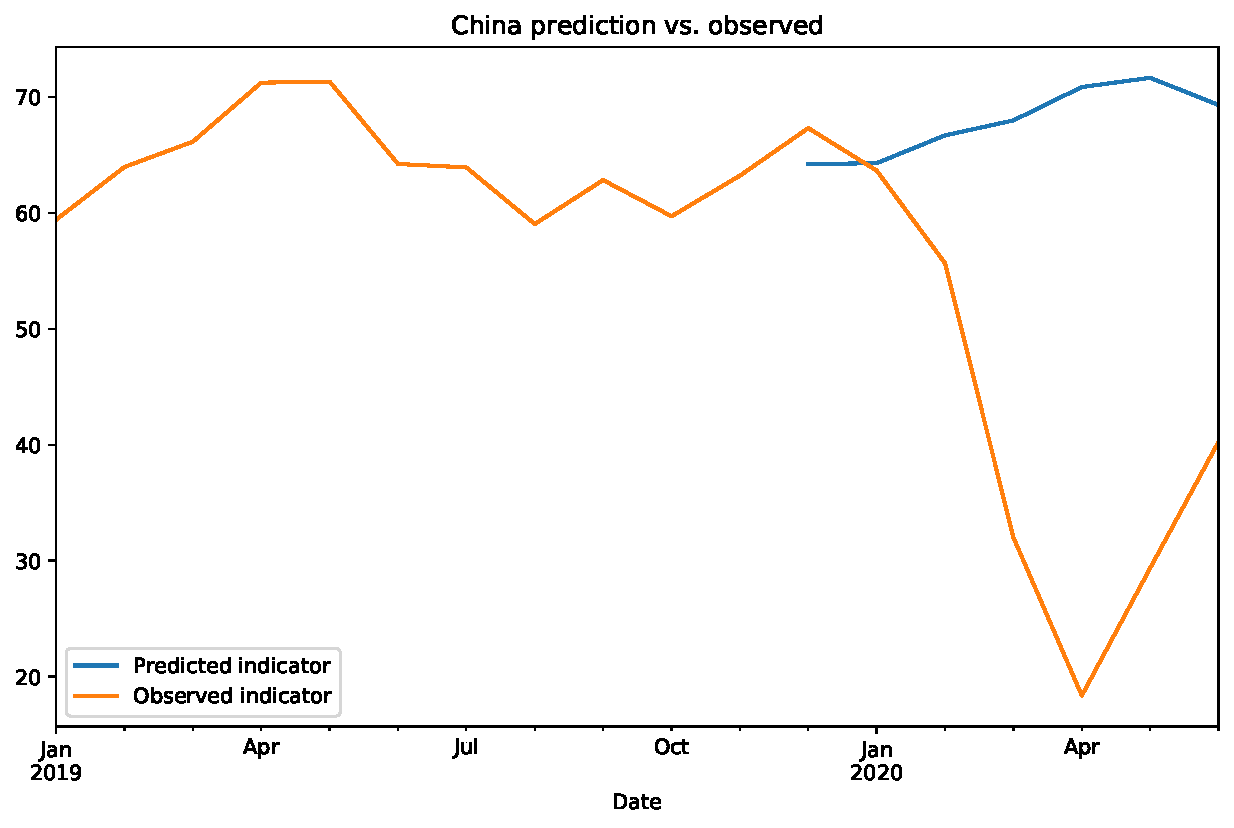
\includegraphics[width=0.4\linewidth]{../power_industry/China_prediction}} \\
	\subfloat[Japan]{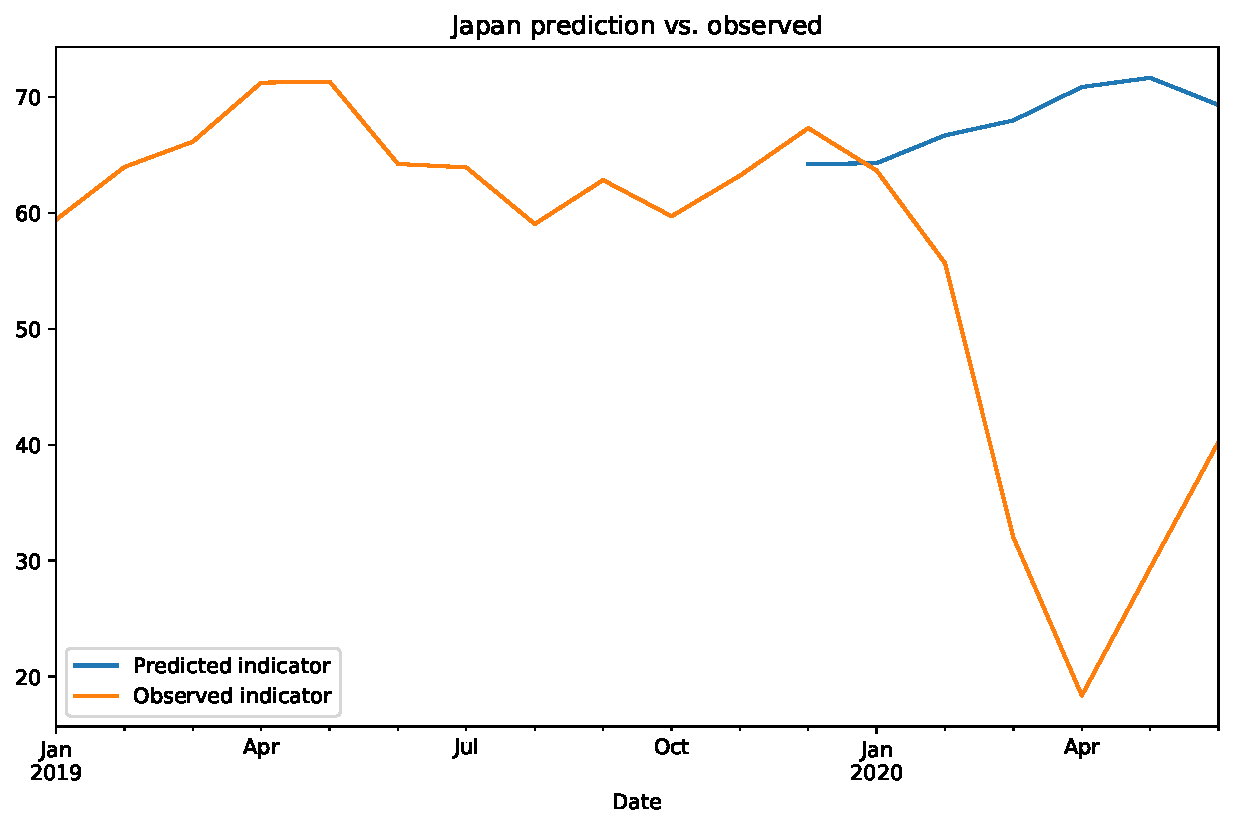
\includegraphics[width=0.4\linewidth]{../power_industry/Japan_prediction}}
	\subfloat[Russia]{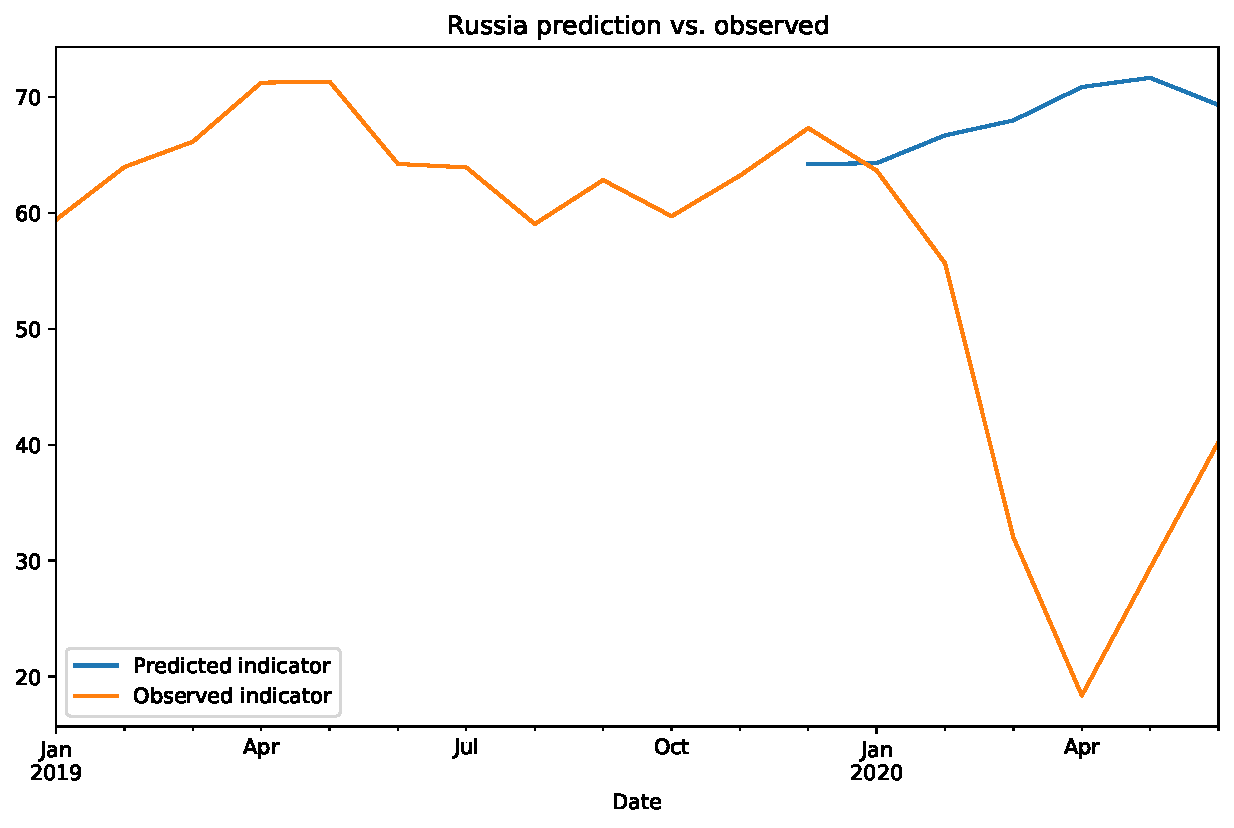
\includegraphics[width=0.4\linewidth]{../power_industry/Russia_prediction}} \\
	\subfloat[Canada]{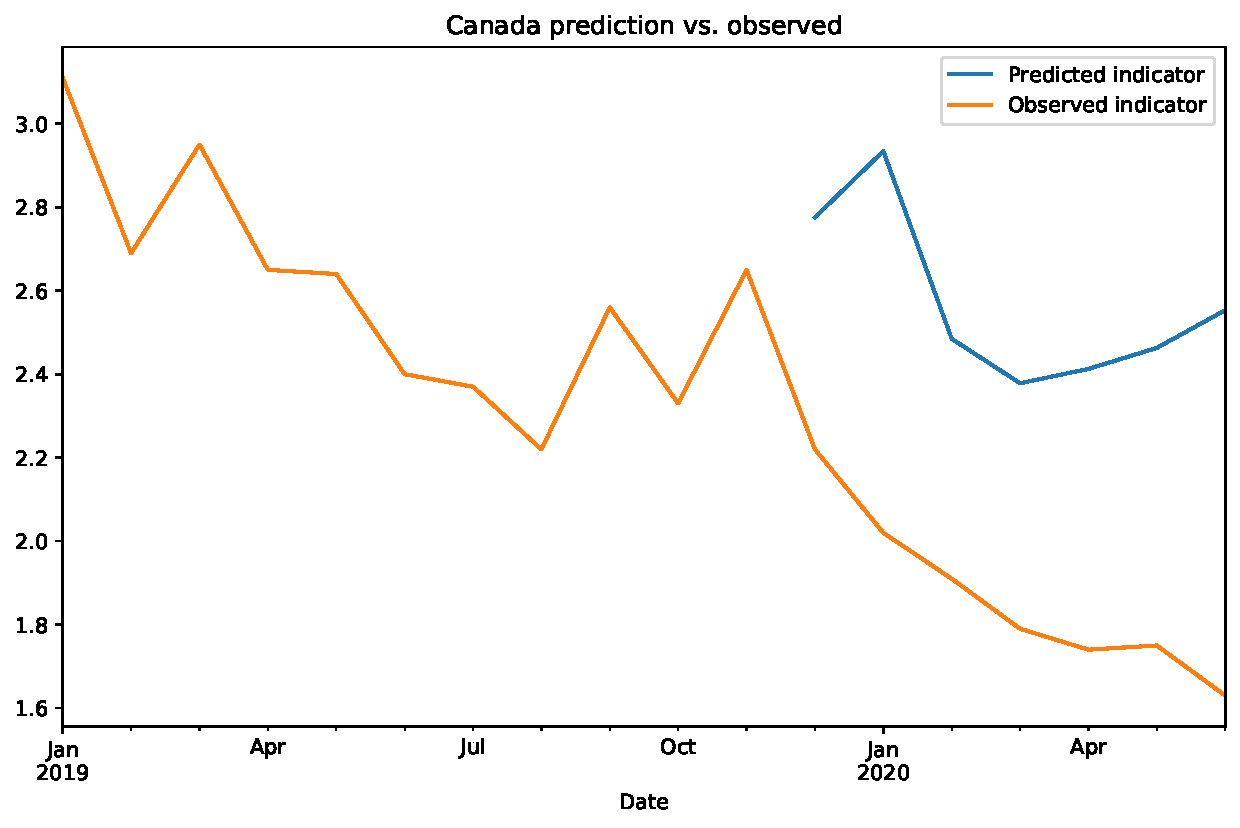
\includegraphics[width=0.4\linewidth]{../power_industry/Canada_prediction}}
	\subfloat[Brazil]{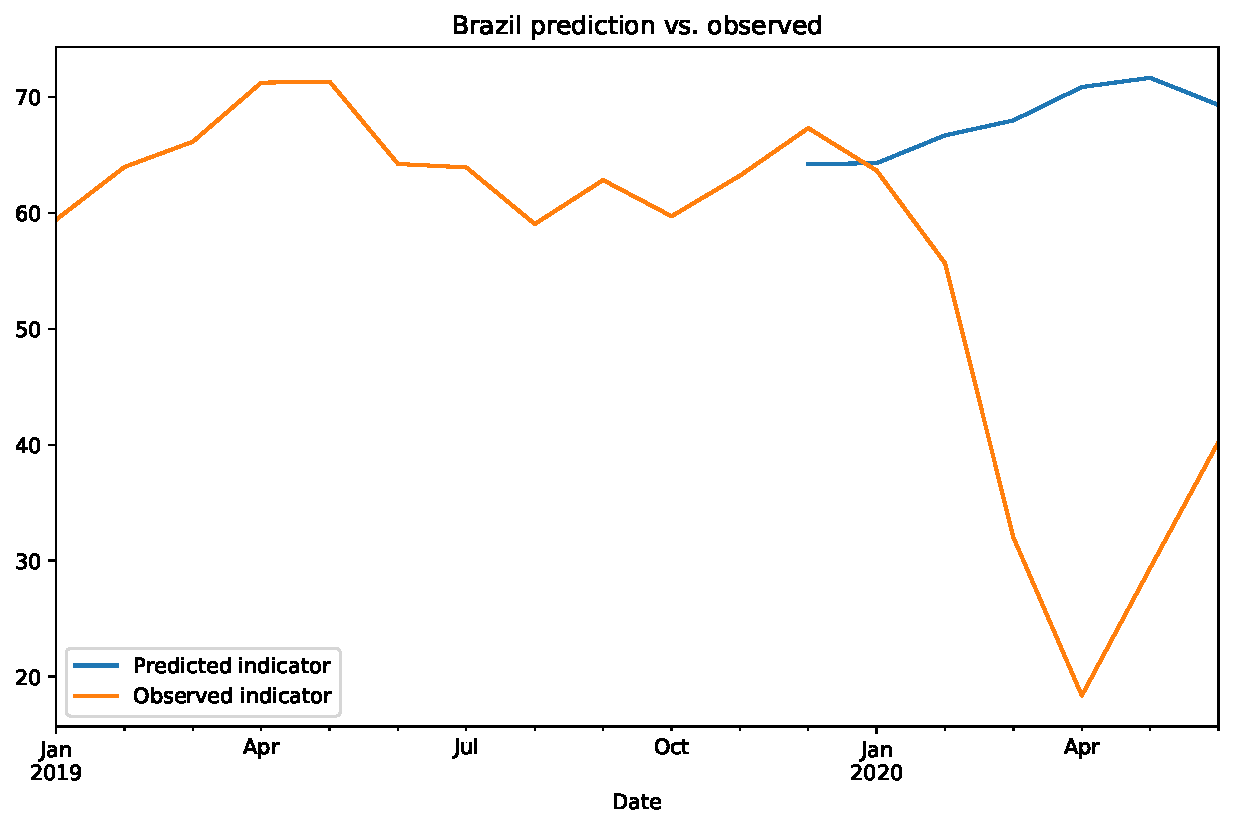
\includegraphics[width=0.4\linewidth]{../power_industry/Brazil_prediction}}
	\caption{Predicted vs real values of selected indicators.}
	\label{fig:sarima}
\end{figure}

In Table \ref{table:change} we show the rate of change for the months we have data. This ratio can be described as:

\begin{equation}
\text{Rate} = \frac{\text{indicator considering COVID-19}}{\text{indicator without considering COVID-19}} = \frac{\text{actual value of the indicator}}{\text{prediction of the indicator}} 
\end{equation}
\begin{table}[h!]
	\centering
	\begin{tabular}{c|cccccccc}
		\hline
		Country & European Union & United States & India & China & Japan & Russia & Canada & Brazil \\ 
		\hline 
		December, 2019 & 0.996 & 0.800 & 1.048 & 1.048 & 1.048 & 1.048 & 0.800 & 1.048  \\
		January, 2020 & 0.998 & 0.688 & 0.990 & 0.990 & 0.990 & 0.990 & 0.688 & 0.990 \\
		February, 2020 & 0.971 & 0.769 & 0.835 & 0.835 & 0.835 & 0.835 & 0.769 & 0.835 \\
		March, 2020 & 0.958 & 0.752 & 0.471 & 0.471 & 0.471 & 0.471 & 0.752 & 0.471 \\
		April, 2020 & 0.927 & 0.721 & 0.259 & 0.259 & 0.259 & 0.259 & 0.721 & 0.259 \\
		May, 2020 & 0.859 & 0.710 & 0.410 & 0.410 & 0.410 & 0.410 & 0.710 & 0.410 \\
		June, 2020 & \textit{No data} & 0.638 & 0.581 & 0.581 & 0.581 & 0.581 & 0.638 & 0.581 \\
		\hline
	\end{tabular}
	\vspace{1em}
	\caption{Rate of change in the indicator.}
	\label{table:change}  
\end{table}

%\paragraph{Conclusion}
Due to the lack of data in emissions of $ CO_2 $, the reliability in our assumptions is based in the correlation with an indicator. Consequently, there are countries which this relation is not very strong and the vector of rate change does not make any sense, since it does not show a reliable situation. 

As mentioned before, non European countries tend to have smaller correlations due to having only two global indicators. In contrast, countries which belong to Europa have four indicators, being two of them unique per country. In results we shown cases with good performance and others which are not optimal, regardless of the region.




\subsubsection{Construction}
%Results
\paragraph{Results}

First, the gridsearch with k fold cross validation was executed to retrieve the best regularization parameter and kernels to reduce overfitting.

For each country the gridsearch provided different optimal kernels and regularization strengths. The resulting parameters are provided in Table \ref{buildings:kernel} together with the resulting scores.

\begin{table}[h!]
	\centering
	\begin{tabular}{clll}
		\hline
		Country & Regularization strength & Kernel & negative RMS error \\
		\hline
		\hline 
		EU & 'C': 10 & 'rbf' &
		-0.67 \\
		United States & 'C': 10 & 'poly' & 
		-0.74 \\
		India &'C': 10 & 'poly' &
		-0.23 \\
		China &'C': 100 &  'rbf' &
		-0.36 \\
		Japan &  'C': 10 & 'rbf' &
		-0.32 \\
		Russia &'C': 10 & 'poly' &
		-0.67 \\
		Canada &'C': 10 & 'rbf' &
		-1.20 \\
		Brazil &'C': 10 & 'rbf' &
		-0.38 \\
		\hline 
		&&& \\
	\end{tabular}
	\caption{Resulting parameters.}
	\label{buildings:kernel}  
\end{table}



\begin{figure}[h]
	\centering
	\subfloat[EU]{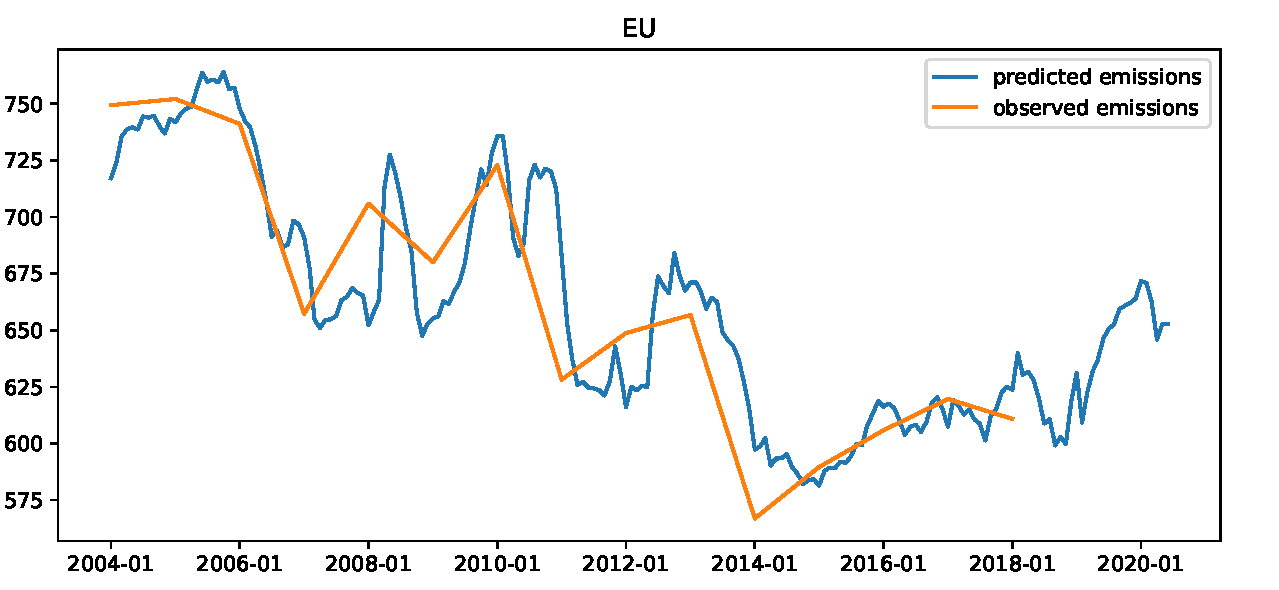
\includegraphics[width=0.5\linewidth]{../buildings/eu}}
	\subfloat[USA]{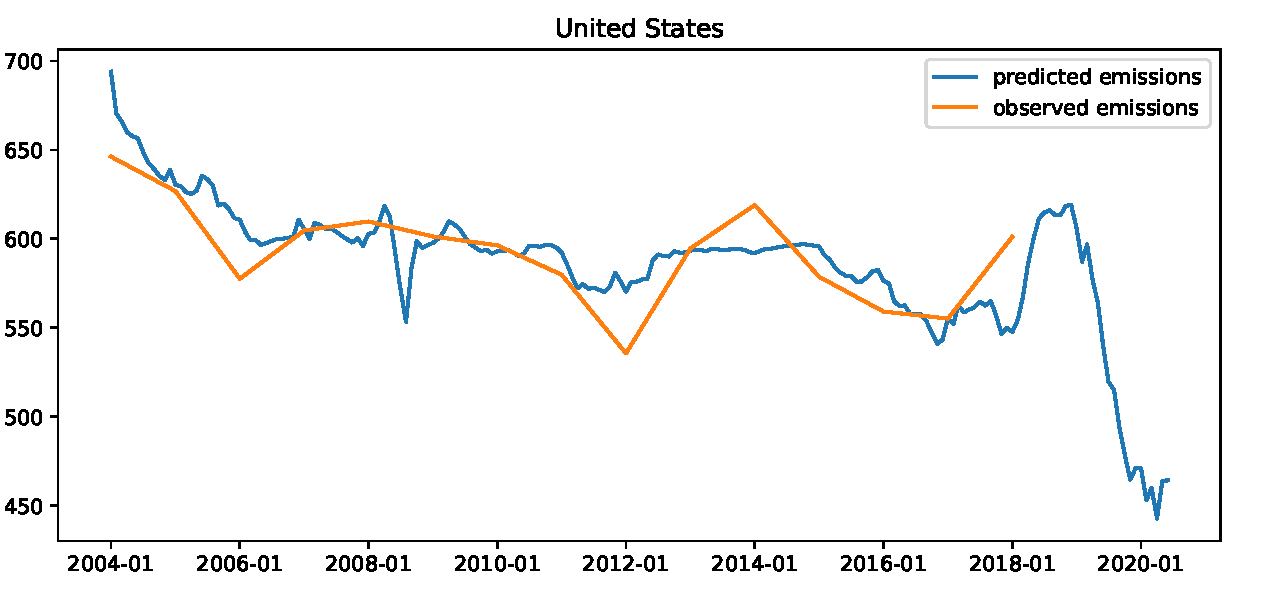
\includegraphics[width=0.5\linewidth]{../buildings/united_states}}\\
	\subfloat[Brazil]{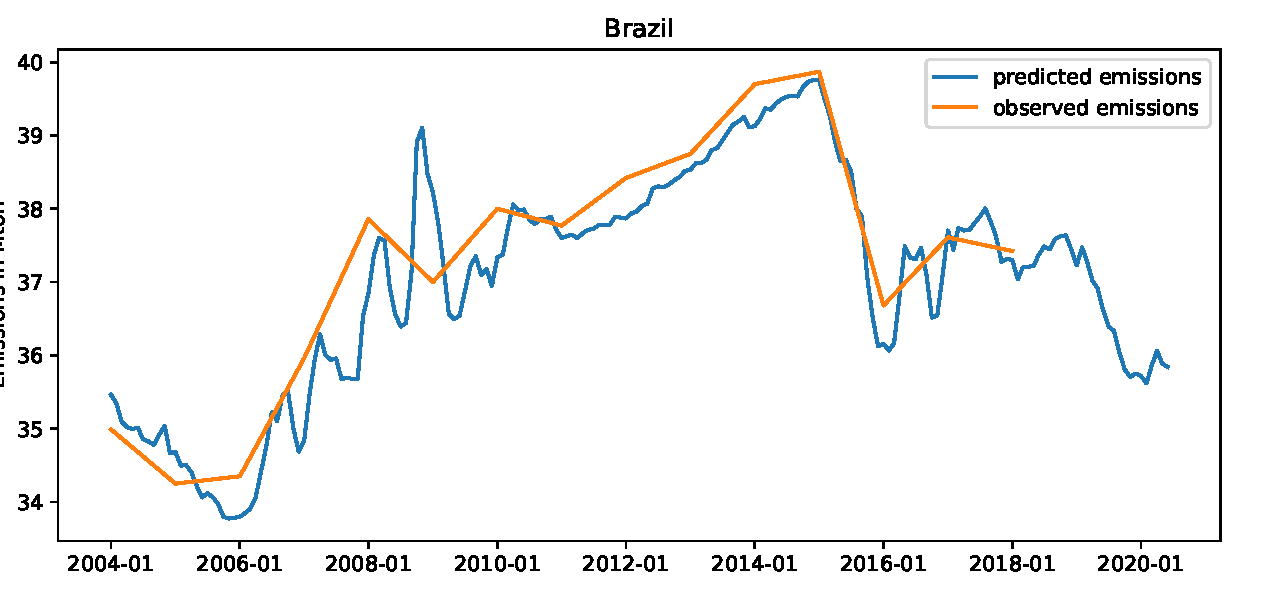
\includegraphics[width=0.5\linewidth]{../buildings/brazil}}
	\subfloat[Russia]{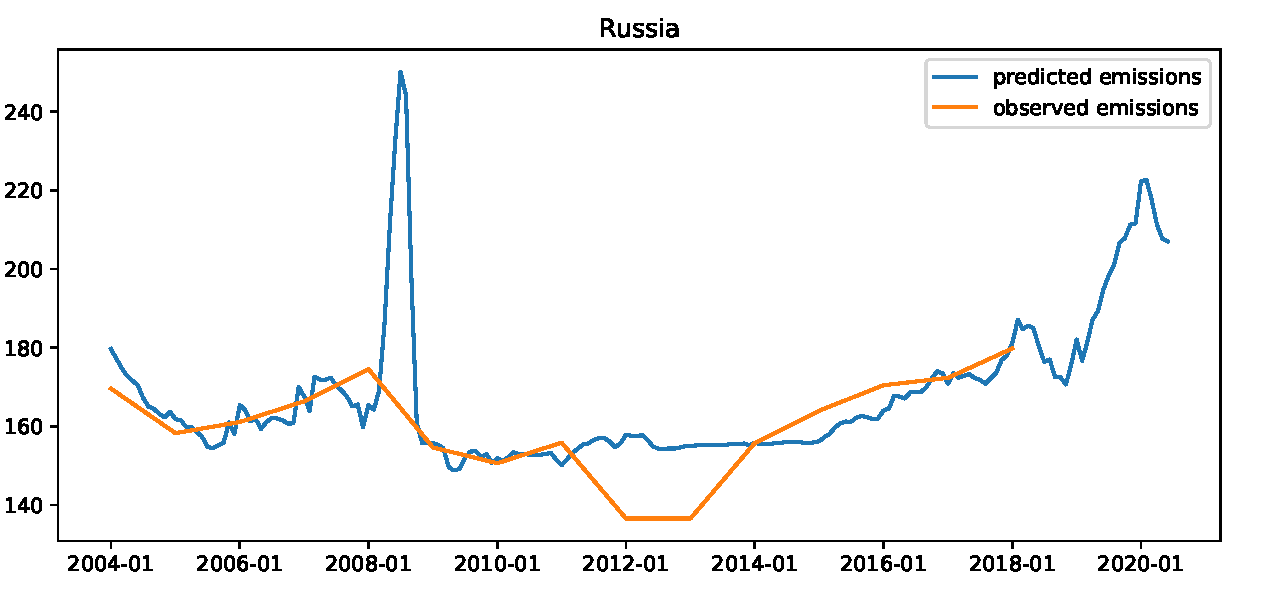
\includegraphics[width=0.5\linewidth]{../buildings/russia}}\\
	\subfloat[India]{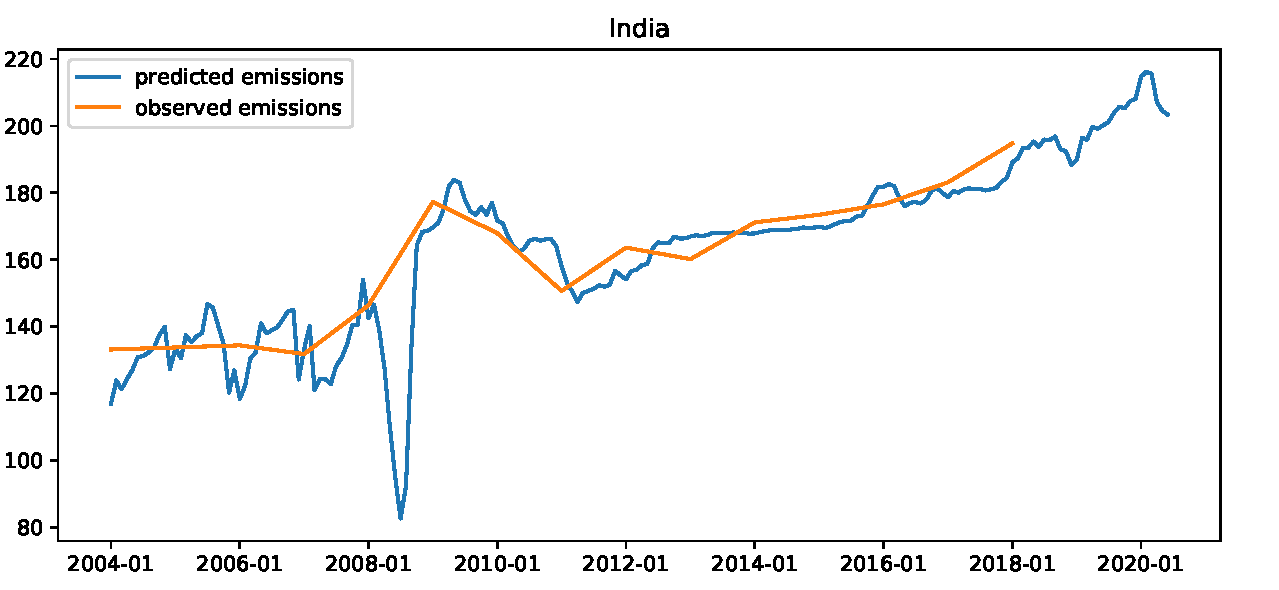
\includegraphics[width=0.5\linewidth]{../buildings/india}}
	\subfloat[Japan]{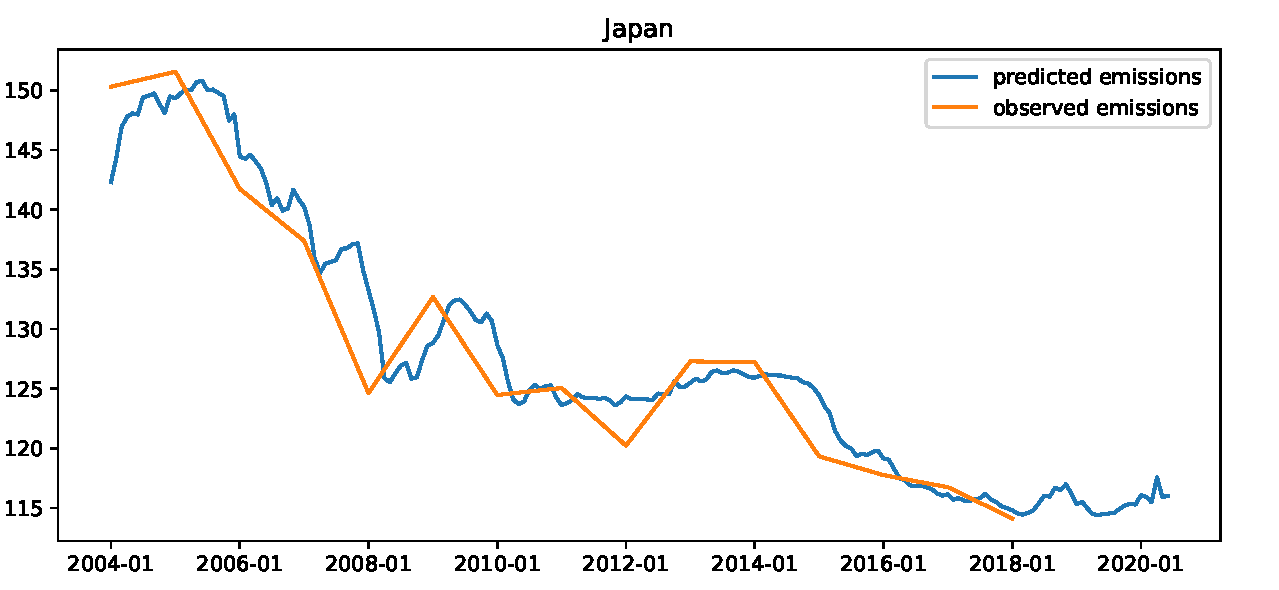
\includegraphics[width=0.5\linewidth]{../buildings/japan}}\\
	\subfloat[Canada]{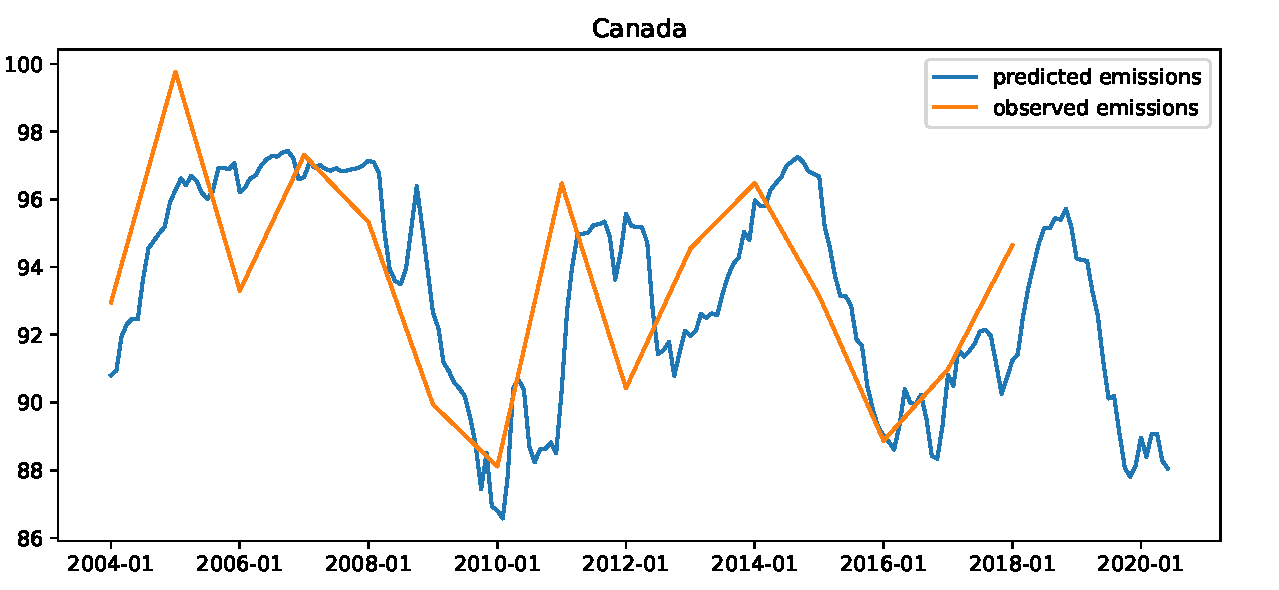
\includegraphics[width=0.5\linewidth]{../buildings/canada}}
	\subfloat[China]{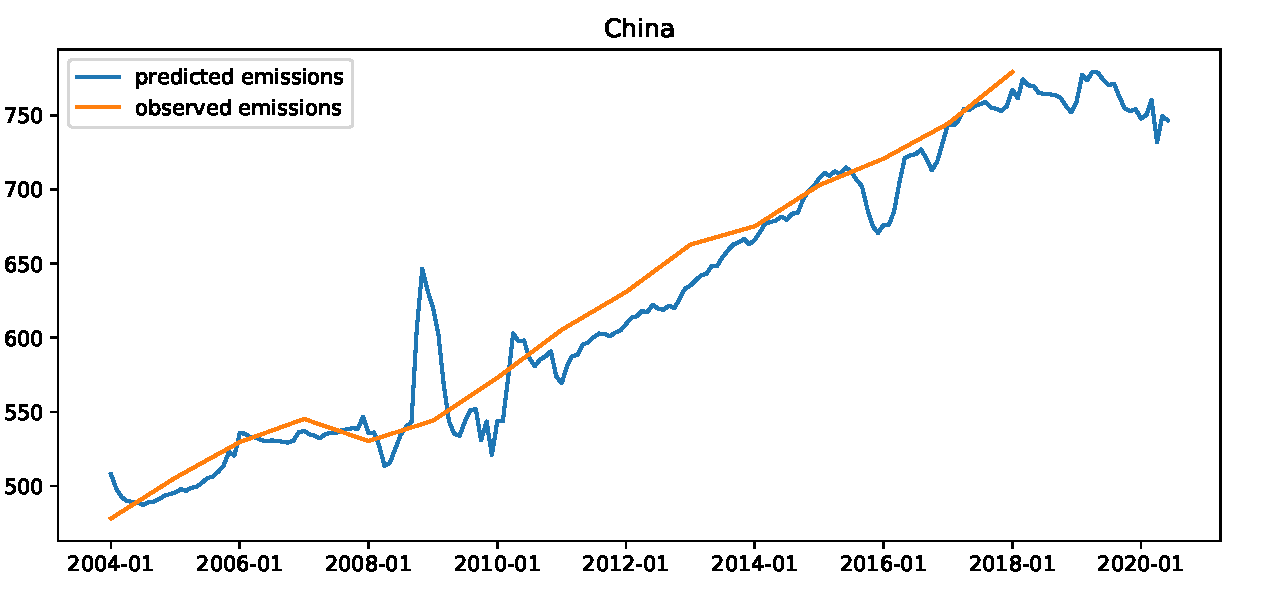
\includegraphics[width=0.5\linewidth]{../buildings/china}}
	\caption{Predicted emissions based on indicators on training set and for 2020.}
	\label{fig:mobility_pred}
\end{figure}	


%Conclusion
\paragraph{Conclusion}

In conclusion, we were able to model the countries sufficiently well. Each country showed an emission drop in the early months of 2020, indicating that COVID-19 had an impact on the indicators and therefore on the overall emissions in the sector.
%todo: scores are lacking

\section*{Observations}

% Task: 

% New Structure:

% Raw Text from previous reports:


With indicators for all sectors, we can now model how the \co emissions for each of the eight countries behaved for the first half of 2020. For that, we combine all sectors for each country according to each sector's contribution.


We provide our result in \autoref{fig:predictedCO2}. The data is seasonality adjusted already, which means that the height of each line directly gives the fraction of \co emissions we would have expected for this month. This is our main result for this Milestone and it completely meets our expectations. We took a lot of different data into account and tried to model \co emissions as accurately as possible with our (limited) resources. Since we took so many different data sets into consideration we think it is fair to assume that we minimized the overall uncertainty. We used a lot of different machine learning models, each one carefully chosen such that we obtain the best results only. 

We still think that we could have done even better with more resources but nevertheless, we are very satisfied with the outcomes of our model so far. We therefore conclude that our model and approach is valid, delivering a result with which we can finally compare COVID-19 case numbers now. This will be done in the next and final Milestone.

\begin{figure}[hb!]
	\centering
	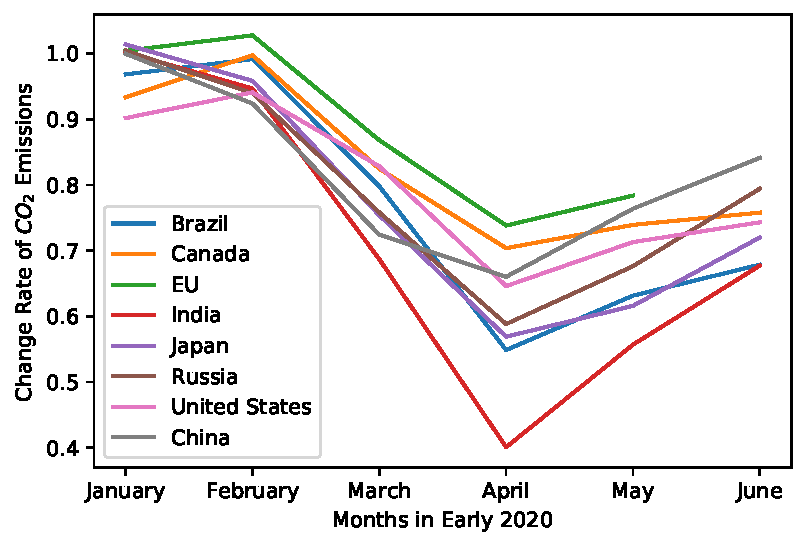
\includegraphics[width=0.7\linewidth]{../predictions/change_rate.pdf}
	\caption{Change of CO2 emissions for each country we consider. As expected, we observe a drop in \co emissions.}
	\label{fig:predictedCO2}
\end{figure}

\subsubsection{Transport}

\paragraph{Result}

Due to the huge size of the project, we had to cut back on some details and make some assumptions. As we could not find out the correct contributions of transit and driving mobility to the \co emissions of this sector, we had no choice but to weigh those two categories equally. We then calculated the monthly average, which lead to the resulting indicators depicted in \autoref{fig:indicator_mobility}. As all data is normalized to the first day of available data, all indicators should start at one. But since we are taking the mean of the first month, one can see small deviations from one for most countries.

For China, we had to assume a curve similar to the others and took mean values of suitable countries and set the mobility to one in months were COVID-9 had no to little impact, like January and June.


\begin{figure}[ht!]
	\centering
	\subfloat[Transit indicator]{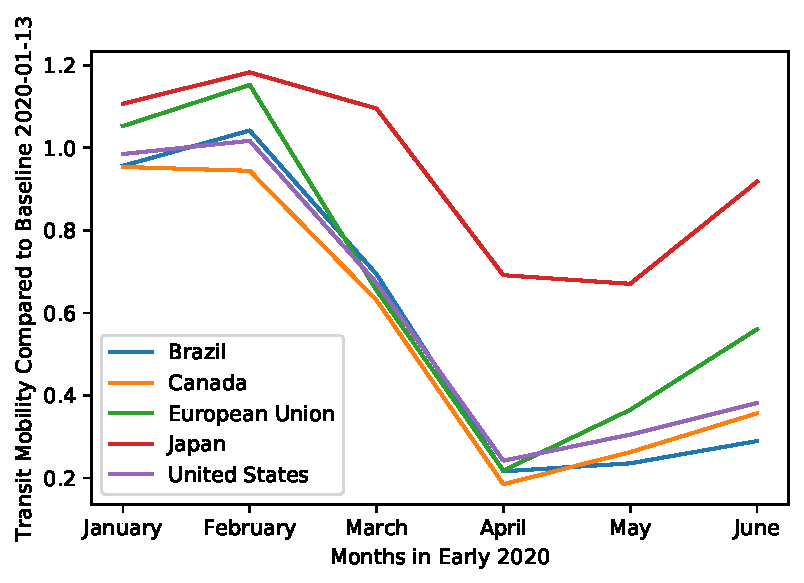
\includegraphics[width=0.48\linewidth]{../predictions/indicator_transit.pdf}}
	\hfill
	\subfloat[Driving indicator]{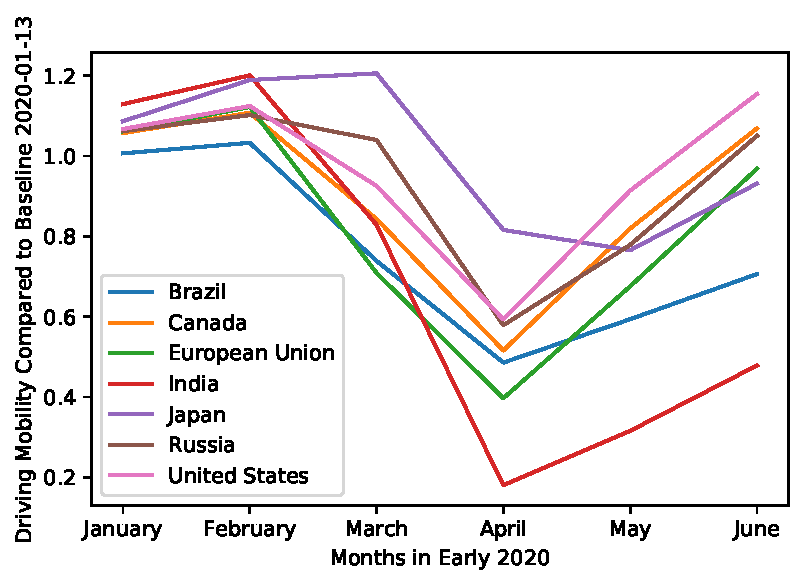
\includegraphics[width=0.48\linewidth]{../predictions/indicator_driving.pdf}}
	\caption{The two \textit{driving} and \textit{transit} mobility indicators before we combine them to one overall mobility indicator.}
	\label{fig:both_mobility_indicators}
	\end{figure}
	
	\begin{figure}[hb!]
		\centering
		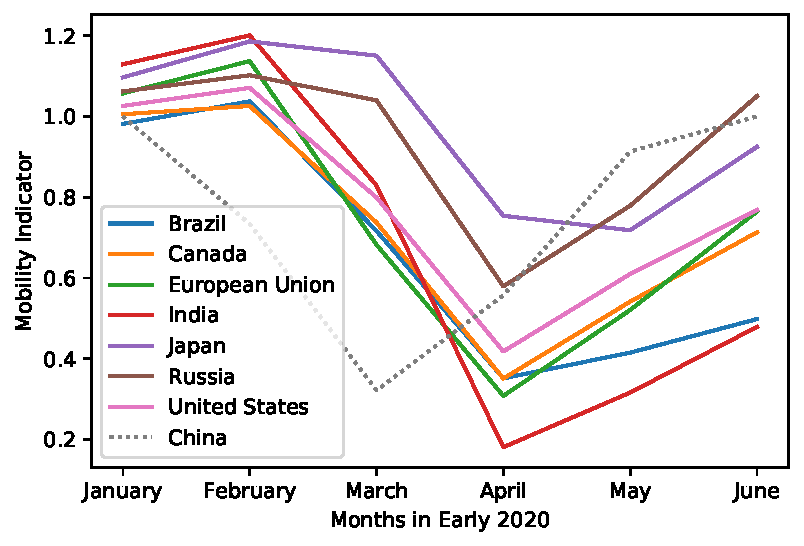
\includegraphics[width=0.7\linewidth]{../predictions/full_mobility_indicator.pdf}
		\caption{Calculated mobility indicator, including China.}
		\label{fig:indicator_mobility}
		\end{figure}
		
		\paragraph{Conclusion}
		
		It is very unfortunate that we have no data on China, as it is the biggest emitter of \co. This definitely has an impact on the validity and accuracy of the mobility indicator and therefore the model. Still, we tried to model China's mobility as accurately as possible. As we can see in \autoref{fig:indicator_mobility}, we assume that China's emission drop earlier than the others, which is a fair assumption as the pandemic started in China.
		
\subsubsection{Other industries}

\paragraph{Results and conclusion}
As seen in \autoref{tab:otherindustry_seasonality}, our calculated seasonality effect is relatively weak, thus adjusting the data does not have a significant impact. This may also be caused by the limited data.
We can see that for most countries a drop in \co emissions for the \textit{other industries} sector can be expected. For China however, we see more or less stable emissions. This surprised us at first. But the stable steel output can be explained with the fact that COVID-19 only hit a very confined region of China in the beginning and was contained more or less successfully later.

\begin{figure}[hbt]
	\centering
	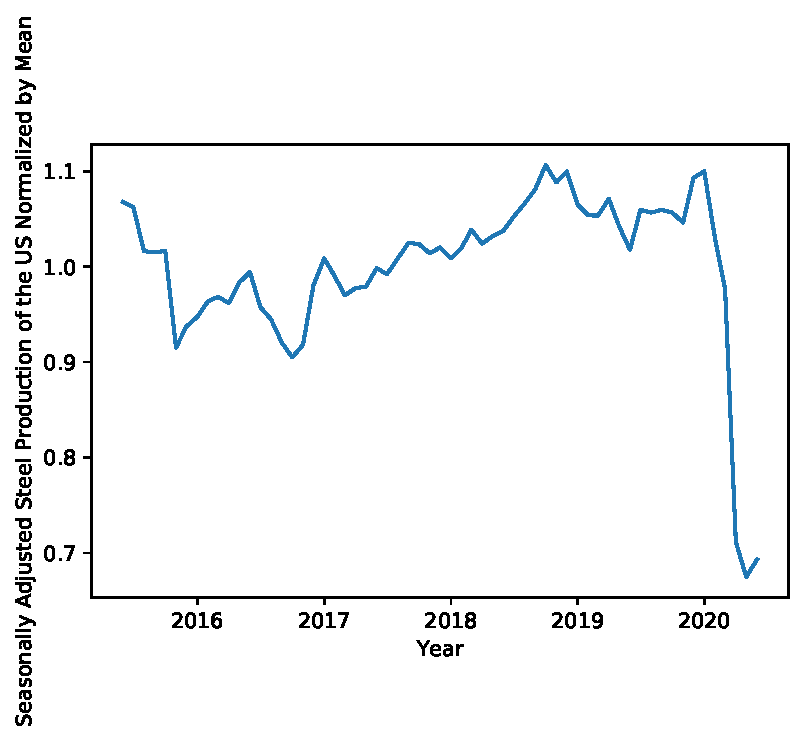
\includegraphics[width=0.69\linewidth]{../predictions/steelUS_seasonadjusted.pdf}
	\caption{Seasonally adjusted steel output of the US, normalized by the mean in the years 2015 to 2020.}
	\label{fig:steelUS_adjusted}
	\end{figure}
	
	
	\begin{table}[h!]
		\centering
		\begin{tabular}{cccccccccccc}
			\hline
			January & February & March & April & May & June & July & August & September & October & November & December\\
			\hline
			\hline
			0.995 & 0.993 & 0.989 & 0.99 & 1.0 & 1.014 & 1.015 & 1.006 & 1.008 & 1.017 & 0.982 & 1.003\\
			\hline &&&&&&&&&&& \\
			\end{tabular}
			\caption{Seasonality trend of steel production in the US.}%todo: source
			\label{tab:otherindustry_seasonality}
			\end{table}
			
			\begin{figure}[h]
				\centering
				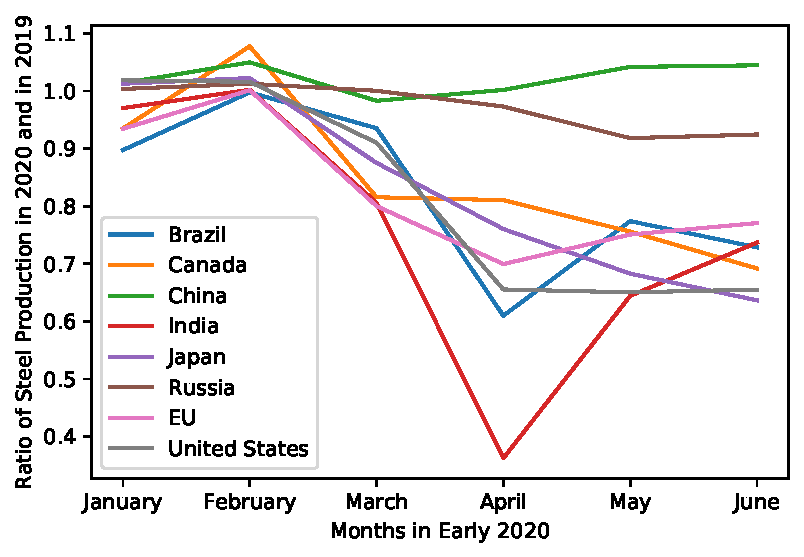
\includegraphics[width=0.7\linewidth]{../predictions/otherindustries_notadjusted.pdf}
				\caption{The indicator of each country without seasonality adjustments.}
				\label{fig:otherindustry_notadjusted}
				\end{figure}


\subsubsection{Other sectors}

\subparagraph{Results}

\begin{table}[h!]
\centering
\begin{tabular}{c c c c} 
\hline
Country & Estimation for 2020 season & State for 1st June 2020 & Percent \\ 
\hline\hline
World & 470.98 & 394.43 & 83.74\% \\
China & 150.43 & 110.32 & 73.33\% \\ 
India & 119.43 & 15.76 & 13.19\% \\
Japan & 7.98 & 5.34 & 66.92\% \\
Brazil & 7.65 & 7.82 & 102.2\% \\
USA & 6.76 & 1.32 & 19.53\%  \\ 
EU & 1.89 & 1.87 & 98.94\% \\
Russia & 0.78 & 0.82 & 105.13\% \\
\hline
&&& \\
\end{tabular}
\caption{The current state of rice crops for the World production and 7 selected areas with a comparison to the estimation for the all 2020 season}
\label{tab:Current_production_rice}
\end{table}

Analyzing \autoref{tab:Current_production_rice} with current data and seasonality of the rice agriculture, we can simply say that there is no impact on this sector during the COVID-19 pandemic. In some countries current state is even higher than the estimated one, whereas in countries where it's lower it basically depends on the seasonality in the particular region. 
		
		
		
\begin{table}[h!]
\centering
\begin{tabular}{c c c c} 
\hline
Country & Estimation for 2020 season & State for 1st June 2020 & Percent \\ 
\hline\hline
World & 362.76 & 345.12 & 95.14\% \\
US & 118.32 & 112.26 & 94.88\% \\ 
Brazil & 135.40 & 131.0 & 96.75\% \\
China & 18.78 & 17.5 & 93.18\% \\
India & 11.39 & 10.5 & 92.19\% \\
Canada & 6.84 & 6.15 & 89.91\%  \\ 
Russia & 5.19 & 4.72 & 90.94\% \\
EU & 3.42 & 2.61 & 76.32\% \\
Japan & 0.58 & 0.34 & 58.62\% \\
\hline
&&& \\
\end{tabular}
\caption{The current state of rice crops for the World production and 8 selected areas with a comparison to the estimation for the all 2020 season}
\label{tab:Current_production_soybean}
\end{table}

Analyzing \autoref{tab:Current_production_soybean} with current data and seasonality of the soybean agriculture, we can say again, without any doubts that there is no impact on this sector. In countries where it is lower it strongly depends on the seasonality period which occurs till the end of July, and the final state can be even higher that the estimated one. 

\paragraph{Conclusion}

In conclusion, whereas both, the livestock and the plant growing has an impact on the \co emission, we can easily notice that COVID-19 does not have impact on the agriculture. Of course there can be some differences between estimated values and the current data because of many factors associated with the global pandemic and lock down, but it has minimal impact in general overview. 
However, there are other concerns related to the pandemic and agriculture. Farmers are afraid that COVID-19 can have an impact not on the production size, but production distribution, and this distribution can contribute to some problems for countries that are dependent on imported crops and for farmers who can't sell their yields. Nonetheless this phenomenon is not a part for our consideration. 
				
\subsection{COVID-19 Data}
\paragraph{Calculating the severity of COVID-19}

Since the purpose of this project is to investigate the correlation between COVID-19 pandemic and  $CO_2$ emissions, we needed a dataset, that provides recent and detailed information on COVID-19 statistics per country. These necessary statistics include number of cases, deaths and recoveries. Accessibility, detail and up-to-dateness of Bing COVID-19 dataset \cite{Bing} made it our primary choice for getting COVID statistics.

Eventually we will need to compare the change in $CO_2$ emissions against the severity of COVID-19 cases in a given country. Since the values in Bing database are absolute, we also need population data for each country. After we combined population information, extracted from \cite{PopulationData}, with COVID-19 statistics, we were able to calculate the severity of COVID-19 in any given country, i.e. deaths and cases per 100,000 people. These rates are visualized in \autoref{fig:covidimpact}. This information is to be compared and correlated with predicted $CO_2$ emissions.

\begin{figure}[h]
	\centering
	\subfloat{\includegraphics[width=0.5\linewidth]{../covid/case rate}}
	\subfloat{\includegraphics[width=0.5\linewidth]{../covid/death rate}}
	\caption{Covid-19 rates for each country.}
	\label{fig:covidimpact}
\end{figure}


\begin{figure}[h]
	\centering
	\subfloat{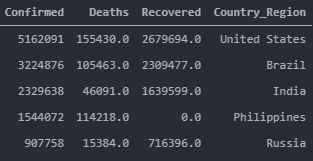
\includegraphics[width=\linewidth]{../covid/bing_top5}}
	\caption{5 countries which have the highest number of cases.}
	\label{fig:bingtop5}
\end{figure}
